\section{Reconstruction using SPINE}

When working with LArTPC detectors, fundamentally, all it returns is a series of voltages that have been read out to the  readout chips.
To get to a physics object from just a number of  voltages, a lot of work has to be done.
This process of converting from raw hits
\footnote{The individual voltages from a channel}
to physics objects is called reconstruction \cite{Dominé_deSoux_Drielsma_Koh_Itay_Lin_Terao_Tsang_Usher_2021}.

\begin{figure}[H]
  %  OWN
  \centering
  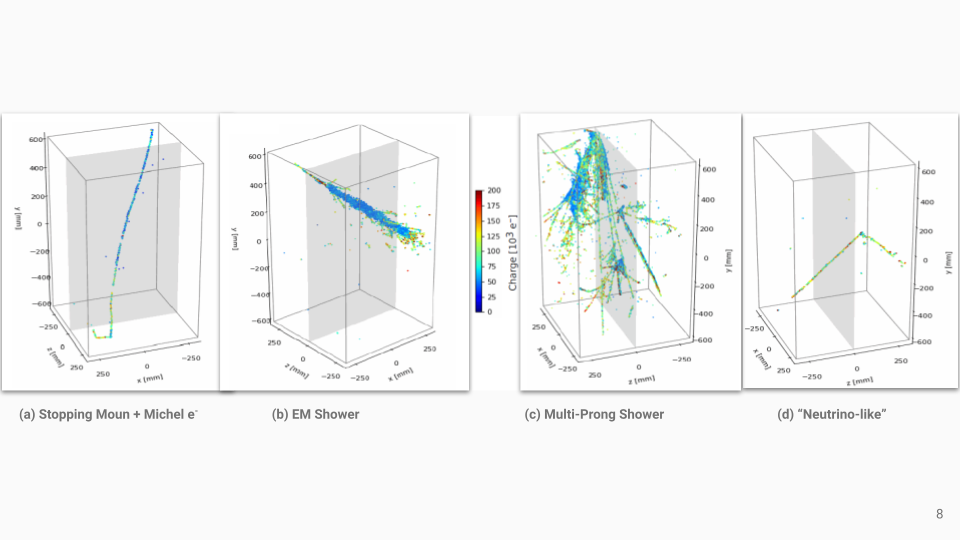
\includegraphics[width=120mm]{figures/mod0Events.png}
  \caption{Some reconstructed events from the module-0 prototype for the DUNE Near Detector}
  \label{mod0Event}
\end{figure}

There are a number of algorithims to do reconstruction of events, oftentimes with their own idiosyncracies, advantages and disadvantages.
The  Scalable Particle Imaging with Neural Embeddings (SPINE) package is one that uses machine learning to perform this reconstruction.

The SPINE  package is designed to work with LArTPC detectors with pixellated charge readout planes.
Traditionally, LArTPC detectors have used wire planes.
These generate a series of 2D pictures rather than  a native 3D image that is generated by a pixellated readout plane.
\footnote{There is an algorithm called  Cluster3D.
  This algorithm processes wire LArTPC data, which consists of three 2D images, to generate 3D points.
  However, this algorithm can introduce inefficiencies, resulting in ghost points—erroneous 3D points that shouldn't be there.}
The modules that are going to be part of the $2 \times 2$  prototype have pixellated planes, SPINE is a useful tool in this context. \cite{drielsma2020clusteringelectromagneticshowersparticle}.

We start with a root file produced either by simulation or with real LArTPC data.
That then gets run through LArCV  which is a C++ library to process LArTPC images.
LArCV processes the root files into what is called a sparse 3D input; just a list of coordinates that correspond to non-zero voxels (3d pixels)

After that, we can engage SPINE proper.

\begin{figure}[H]
  % https://github.com/DeepLearnPhysics/spine?tab=readme-ov-file  \centering
  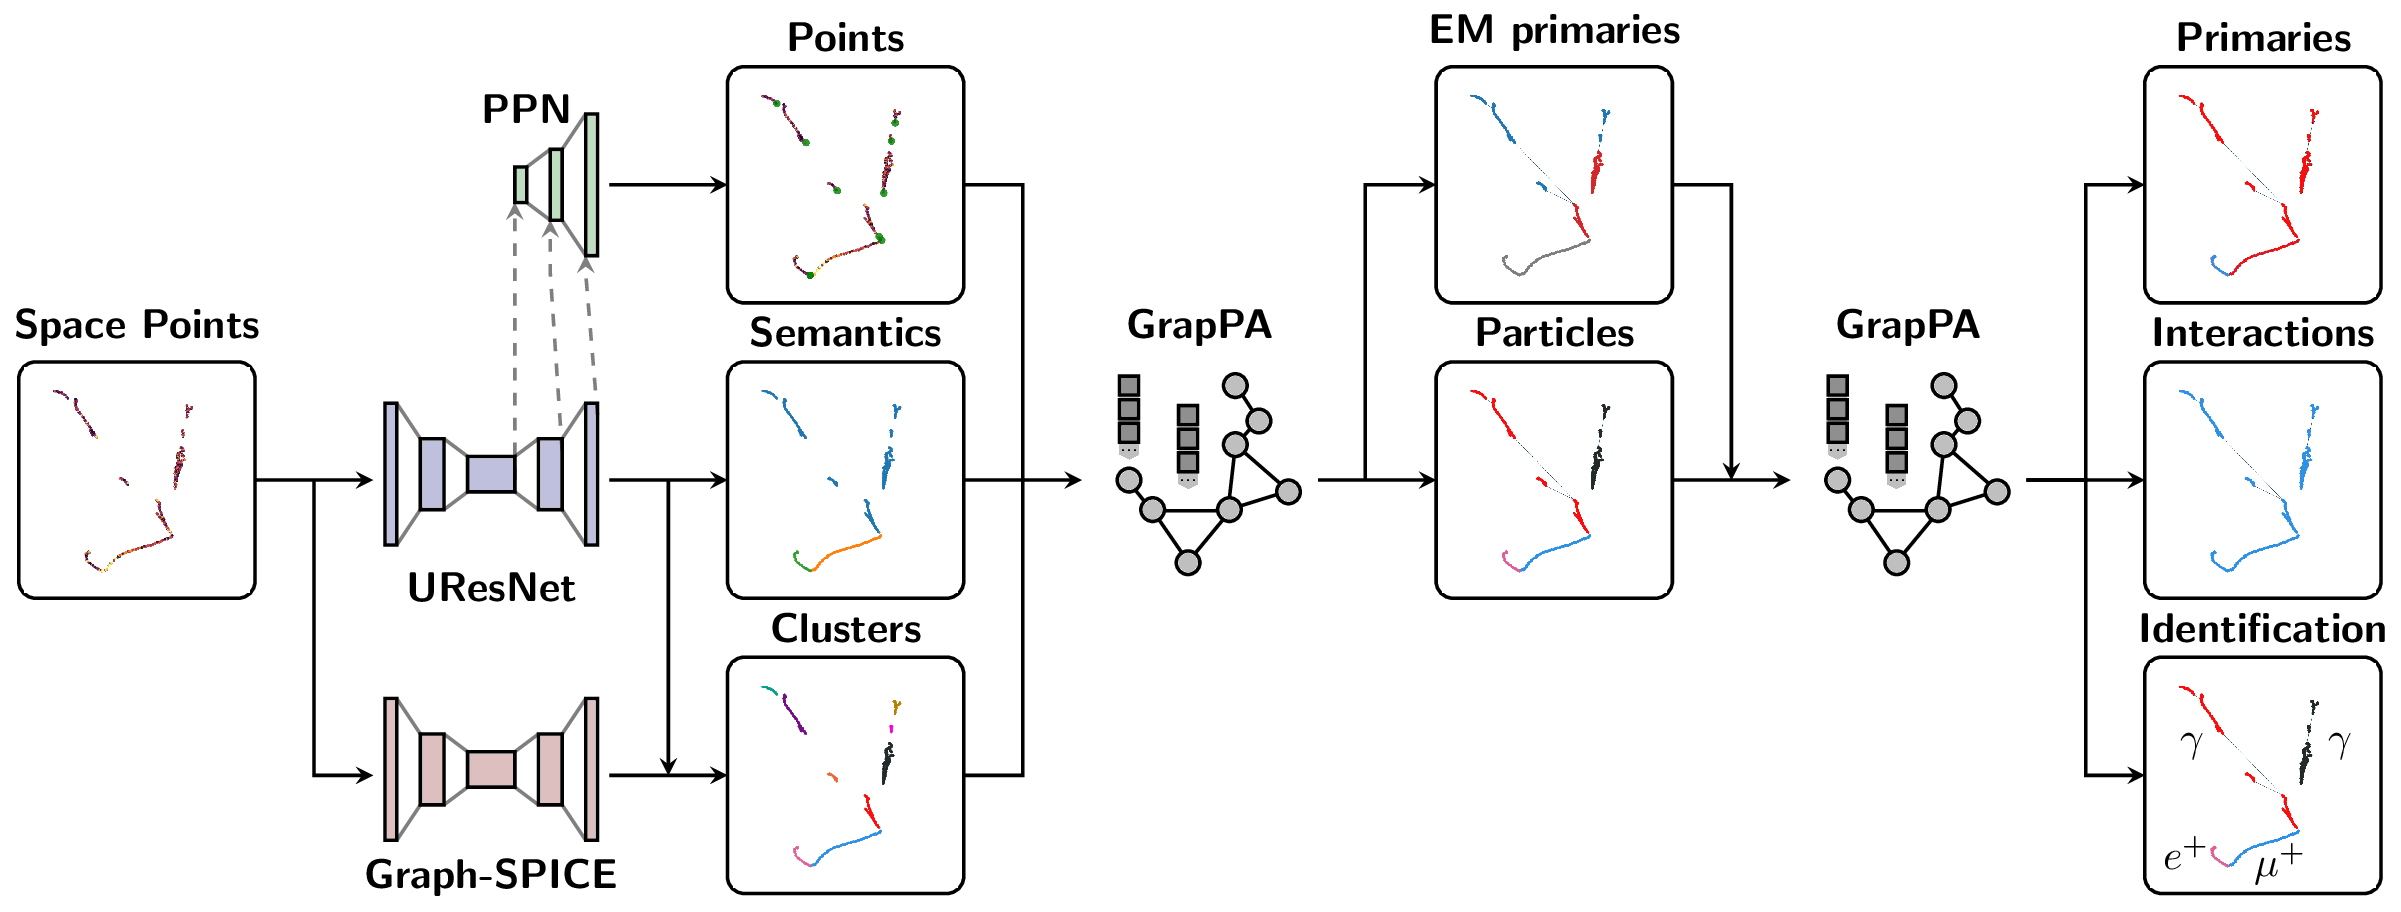
\includegraphics[width=120mm]{figures/spineSchematic.png}
  \caption{Overview of the SPINE schematic\cite{SPINE_schematic}}
  \label{spineSchematic}
\end{figure}

SPINE consists of a number of machine learning models stitched together, working in concert to get from raw hits to reconstructed outputs.
Let's break down each of the parts in turn.

\subsection{Semantic Segmentation and PPN}

\subsection{Particle Clustering}

Once the semantic segmentation is done, their results get passed onto the spice GNN.
The purpose of this GNN is to group different voxels together if they belong to the same shower or track.
The SPICE (Sparsity-preserving Invariant Convolutional Embedding) model is a novel approach designed to address challenges in graph-based learning by leveraging sparsity and invariance principles.
At its core, SPICE utilizes convolutional operations that preserve the structural sparsity of graphs, which is crucial for efficiently processing large-scale and complex graph data.
Lucky for us, neutrino events are incredibly sparse.
By maintaining sparsity, SPICE reduces computational overhead and memory usage, making it scalable to larger graphs.
The invariant convolutional embeddings produced by SPICE ensure that the model is robust to transformations and perturbations in graph structures, such as node and edge additions or deletions, thereby enhancing its generalization capabilities.

In practical terms, SPICE integrates several advanced techniques to optimize graph learning tasks.
The model incorporates a sparse convolutional layer that operates directly on the non-zero elements of graph adjacency matrices, bypassing the need for dense matrix operations that can be computationally expensive.
Additionally, SPICE applies invariant transformations that allow the network to remain effective even when the graph undergoes structural changes.

\begin{figure}[H]
  % 
  \centering
  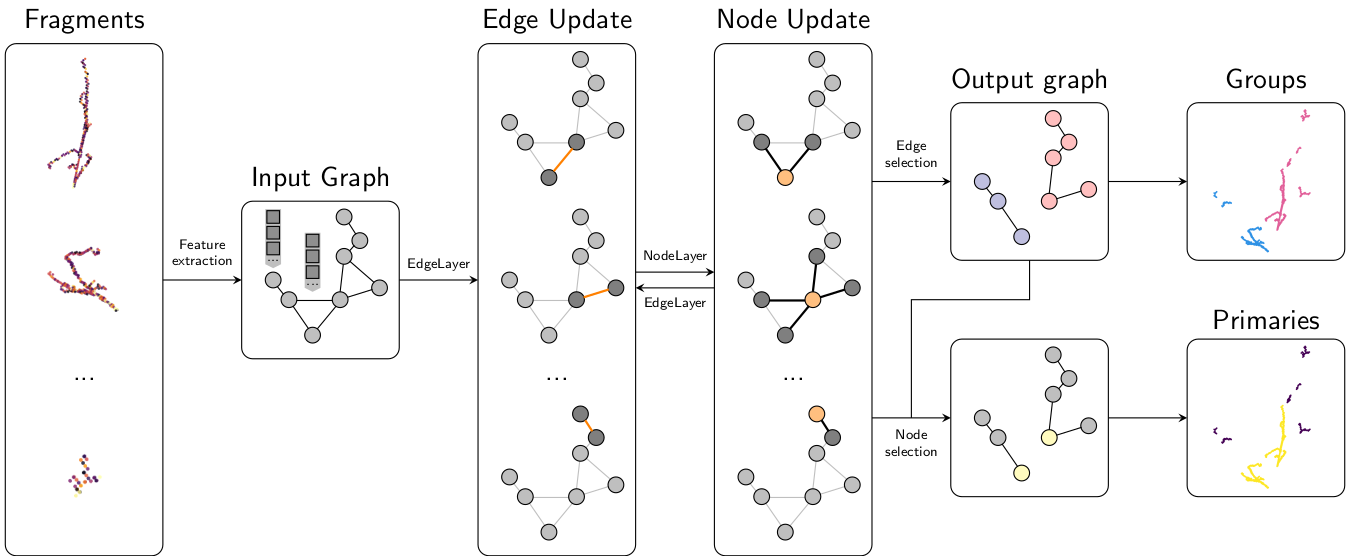
\includegraphics[width=120mm]{figures/gnn.png}
  \caption{Architecture of the clustering GNN}
  \label{gnn}
\end{figure}

This clustering is done in separate parts between the tracks and showers before coming together to cluster interactions.

\begin{figure}[H]
  % OWN
  \centering
  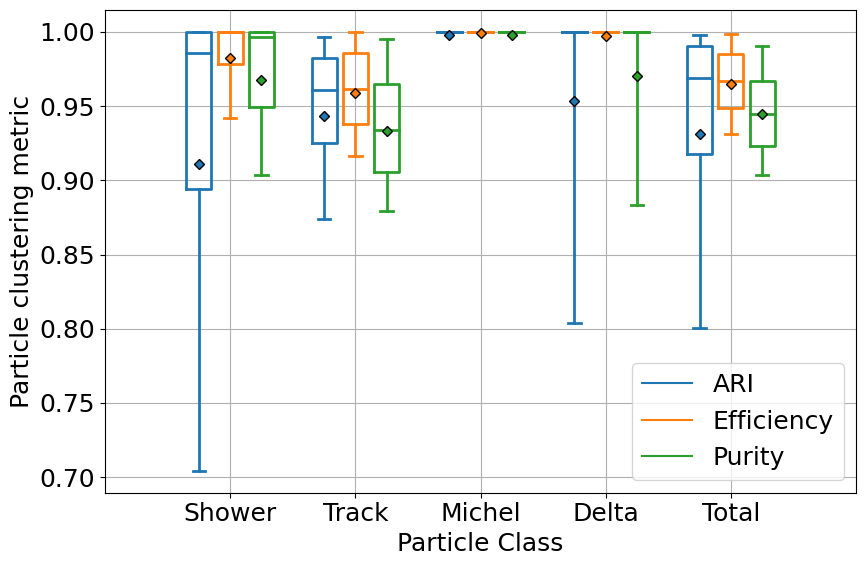
\includegraphics[width=120mm]{figures/clusteringPerformance.png}
  \caption{Box and whisker plot showing performance of clustering}
  \label{clusteringPerformance}
\end{figure}



\subsection{Particle Identification}

Now that things are clustered properly, we move on to do particle identification like in figure \ref{pidEvent}.

\begin{figure}[H]
  % OWN
  \centering
  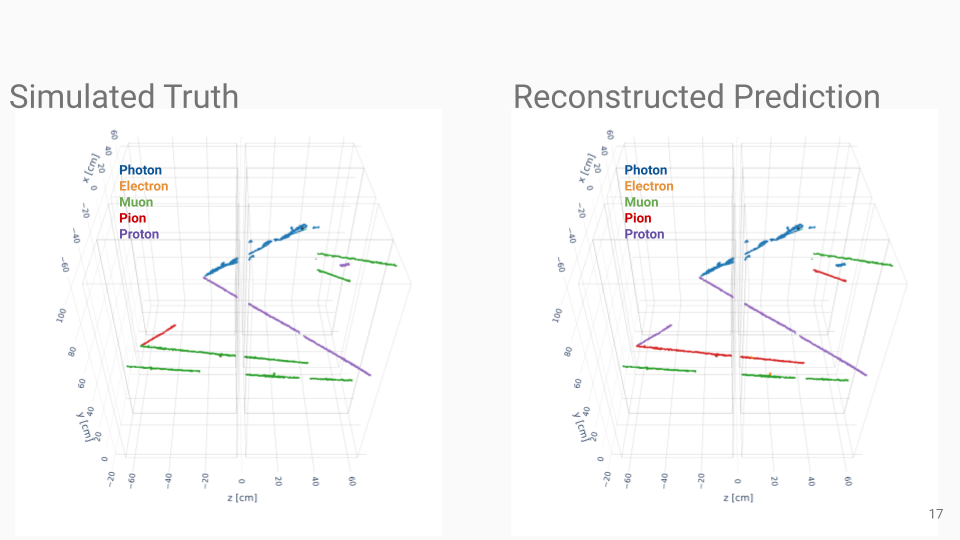
\includegraphics[width=120mm]{figures/pidEvent.png}
  \caption{Particle ID Event display comparing monte carlo truth and reconstructed prediction}
  \label{pidEvent}
\end{figure}

This is done through the Graph Partitioning and Aggregation (GrapPa GNN.GrapPa innovates by combining partitioning and aggregation techniques to handle massive graphs efficiently.
It first partitions the input graph into smaller, manageable subgraphs, ensuring that computational resources are allocated more effectively.
These partitions are then processed independently through GNN layers, which helps in capturing local graph structures without overwhelming the system's memory.
The aggregation step combines the results from these subgraphs, allowing the model to capture global dependencies and maintain a comprehensive understanding of the entire graph's topology.
This approach strikes a balance between efficiency and expressiveness, making it particularly useful for applications with large and complex graph data.

The GrapPa framework also integrates advanced techniques such as hierarchical pooling and dynamic batching to further enhance its scalability and performance.
Hierarchical pooling enables the model to learn and propagate information across different levels of graph granularity, while dynamic batching adjusts the processing load according to the current computational demands.
These features contribute to GrapPa's ability to generalize well across various graph sizes and structures, addressing key limitations of traditional GNNs which often struggle with scalability and efficiency.

\begin{figure}[H]
  % OWN
  \centering
  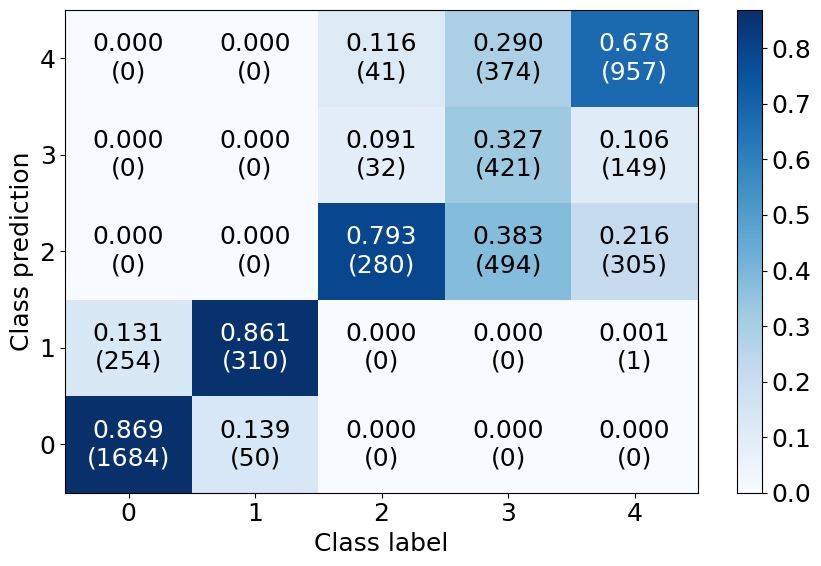
\includegraphics[width=120mm]{figures/pidPerformance.png}
  \caption{Confusion Matrix showing performance of Particle Identification}
  \label{pidPerformance}
\end{figure}

GrapPa tries not only to identify the individual particles but also runs a binary classifier to see if the particle is a primary or secondary.














